\documentclass{article}
\usepackage[utf8]{inputenc}

\title{Introduction to Convolutional Neural Networks}
\author{Mihir Patel}
\date{November 2017}

\usepackage{natbib}
\usepackage{graphicx}
\usepackage{mathtools}          %loads amsmath as well
\usepackage{tikz}
\usepackage{pgfplots}

\begin{document}

\maketitle

\section{Perception: Images}
For humans, perception, especially from visual input, is something we learn very quickly and are very good at. By contrast, computers struggle to understand images in a generalize context and process them. This is because the amount of information is enormous. From just a single 1080p picture, we have over 6.2 million data points, consisting of 3 color channels from approximately 2,073,600 pixels. From this information, it is very difficult to make a claim such as this image is a picture of a dog as a simple change, such as a mirror reflection, basically changes all of the values in the image.

\section{Neural Networks in Images}
The goal then is to apply neural networks and machine learning to images. The idea is that compared to a decision tree or a very rigid approach, the neural network can learn the semantic meaning of the information and labels. In theory, this works wonderfully. Neural networks contain everything we need to learn patterns and have been shown to be highly successful at many basic tasks. However, we quickly encounter the two big problems in machine learning. Firstly, this requires a massive amount of annotated data, which is difficult to obtain. While we could learn anything, it would require a lot of information. Secondly, it is extremely computationally expensive to learn this and the depth of the networks required makes this approach basically unfeasible.

\section{Convolutional Layers}
The issue with neural networks is that they disregard spacial benefits. Two pixels next to each other have more correlation than two pixels on the opposite side of an image. Neural networks feed each pixel into a neuron that must then learn each of these connections, which is a waste of computational power and could be difficult to learn. In order to account for this, we use convolutional layers.

\section{Convolutional Filters}
\begin{center}
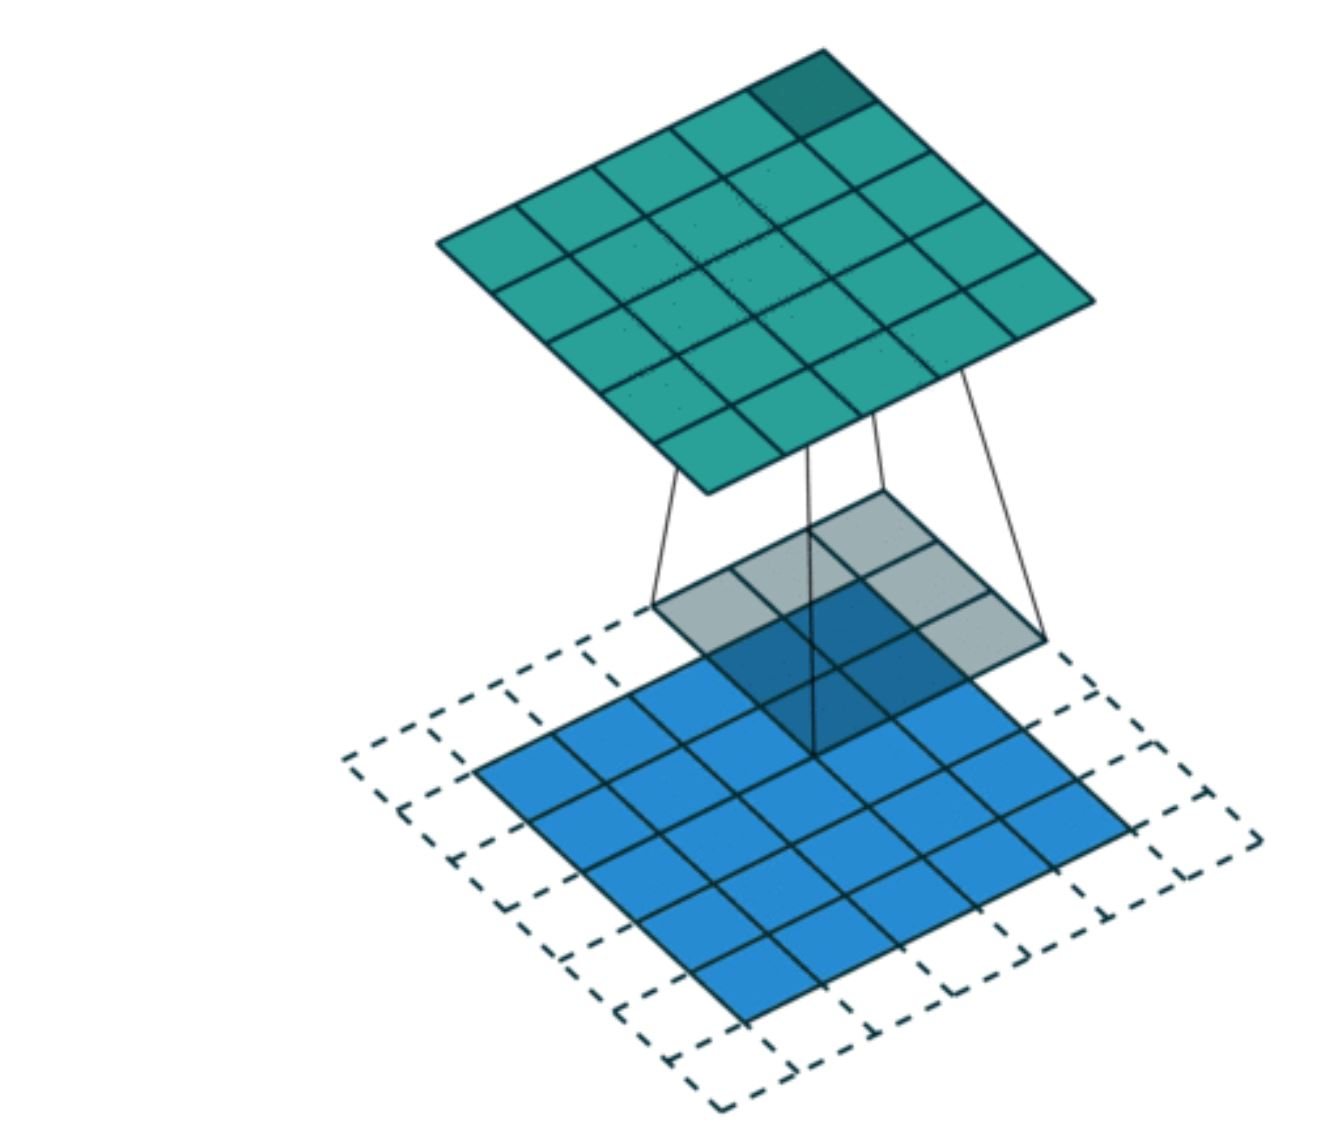
\includegraphics[scale=0.5]{convgif}
\end{center}
\subsection{Definition}
Convolutional layers first start with filters, which are commonly called kernels. Each filter is a matrix of weights that are built to learn a certain pattern. At each location, the filter checks to see if a specific feature, such as a line or a curve exists. Using backpropagation, we can tune the weights in the kernels and have it learn specific features.

\section{Example Filter}
\begin{center}
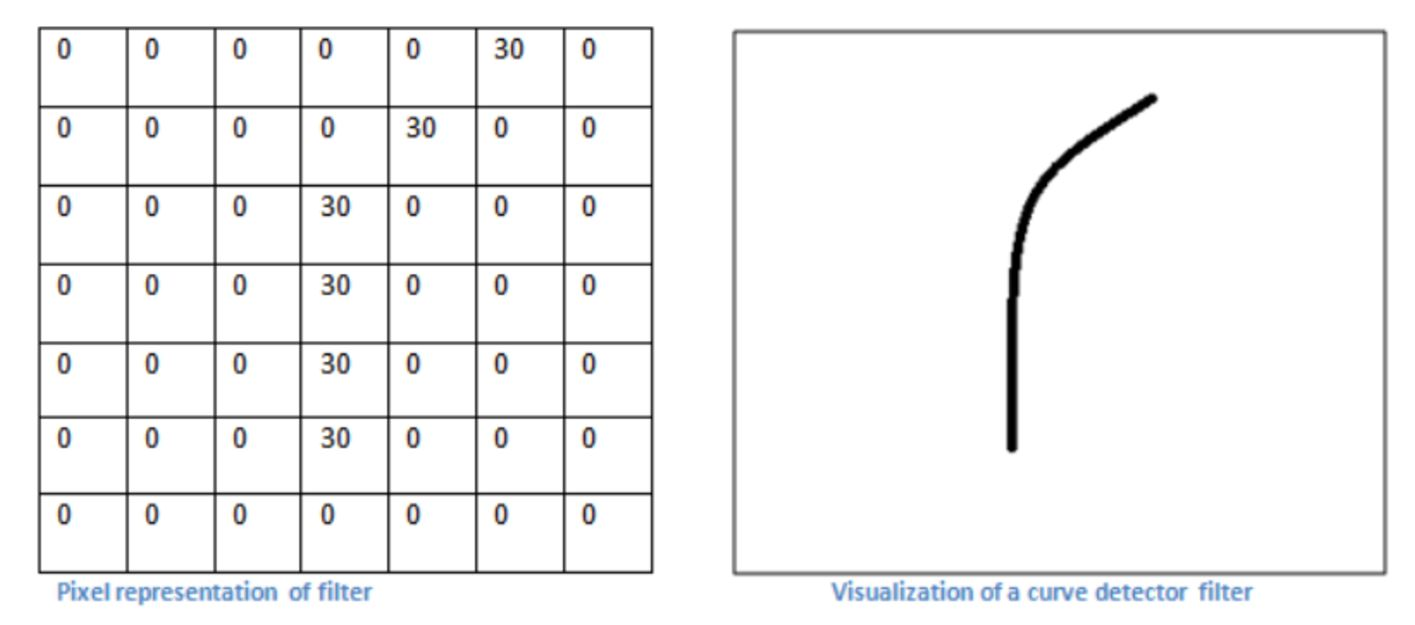
\includegraphics[scale=0.5]{filter}
\end{center}
\subsection{Definition}
As we see here, when this filter finds an image similar to the one on the right, the high values in the filter line up with the shape in the image, causing the filter to "detect a feature". The sum of the multiplication of the matrix and the image (non-matrix multiplication) is passed as the output to the activation function.

\section{Building Layers}
\begin{center}
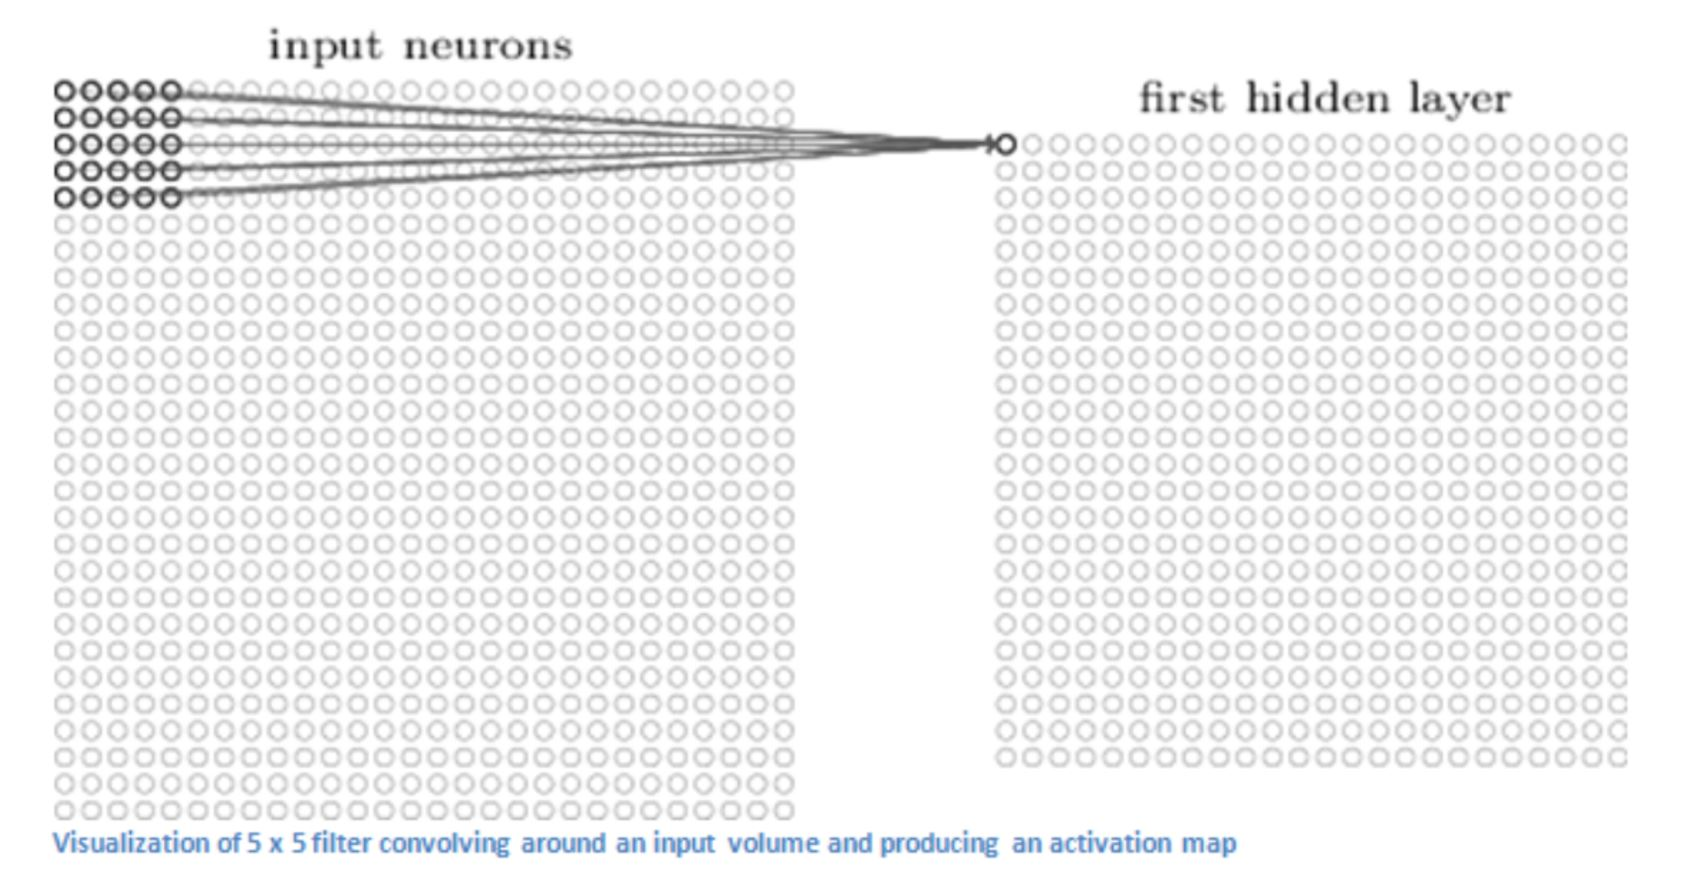
\includegraphics[scale=0.5]{Capture}
\end{center}
\subsection{Definition}
To create a convolutional layer, each filter is applied over the region of the image and the output is mapped to a second layer. Each point tells you whether that feature was detected in a certain location or not. However, since we want to extract multiple features, the subsequent hidden layers also have a z-dimension, with each level in the z-dimension consisting of a different feature. If I created a convolutional layer with 64 features, then 64 of the hidden layers on the right would be stacked together. And that solves our problem of effectively structuring our network! Essentially what we have done is restructured a layer so that connections between neurons far away don't exist and our network doesn't waste time learning that these are meaningless.

\section{ReLU Activation}
So how do we handle activations with these networks? It turns out that sigmoids do work fine. However, they are very slow and cause lots of problems in deep networks, such as vanishing gradient. To handle this, we use the ReLU activation function, which stands for rectified linear unit. We will cover more into this later, but the short answer is that it has a very simple derivative that is constant so we can always maintain our gradient with respect to the error. It does cost us all negative values, which are disregarded, but it turns out to not be too significant.
\[
  y =
  \begin{cases}
                                   0 & \text{if $x < 0$} \\
  x & \text{if $x > 0$}
  \end{cases}
\]

\section{Pooling Layers}
Now, even with all these optimizations, convolutional layers produce a lot of data, if we look for many features, we greatly increase the size of the subsequent hidden layer. However, a lot of this information isn't very useful. For example, while it is important that a curve is in the top right, its exact pixel location isn't as important. To remove this extra information, we use pooling layers.

\section{Max Pooling}
\begin{center}
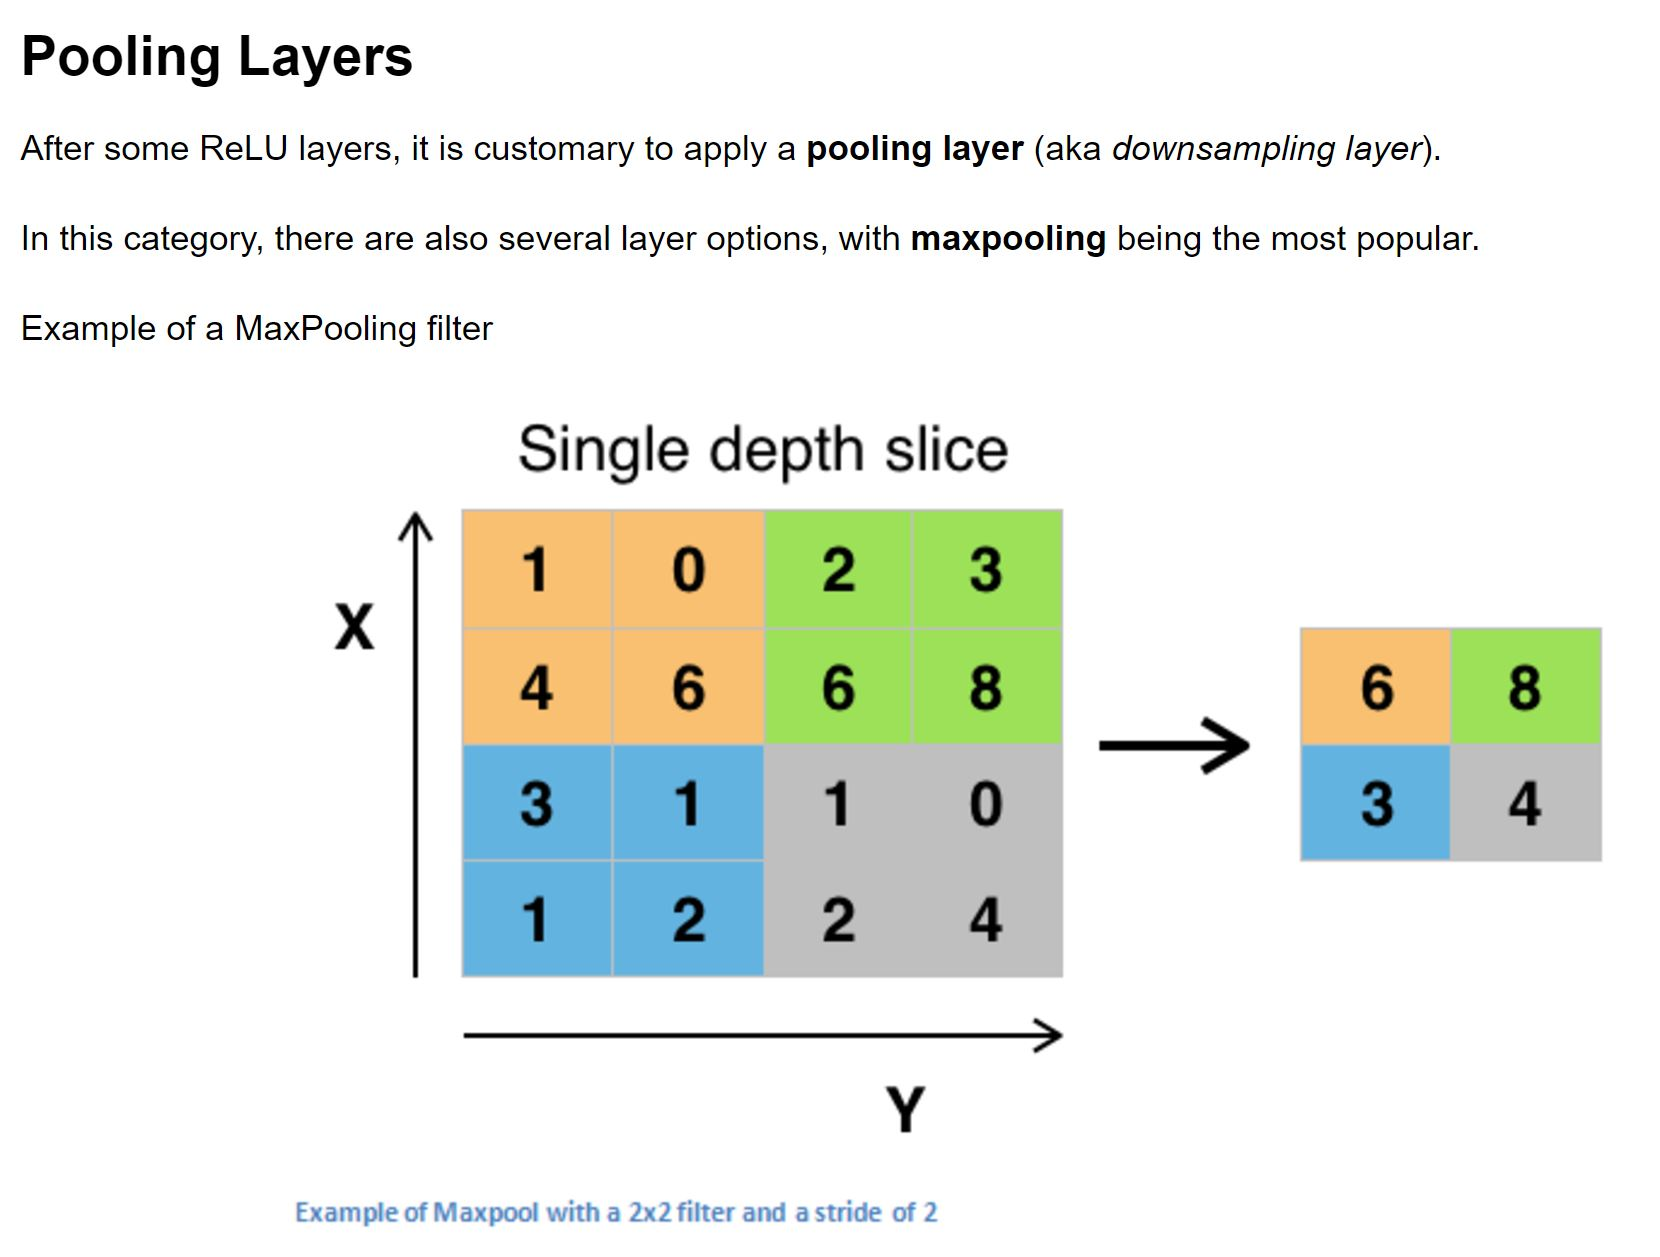
\includegraphics[scale=0.5]{pooling}
\end{center}
\subsection{Definition}
The way pooling layers work is that they take the highest value in each region and only track that. This removes the exact pixel location information and actually helps in making the network more generalizable while decreasing data by 1/4! With this, we can train our networks much, much faster.

\section{Putting it all Together}
\begin{center}
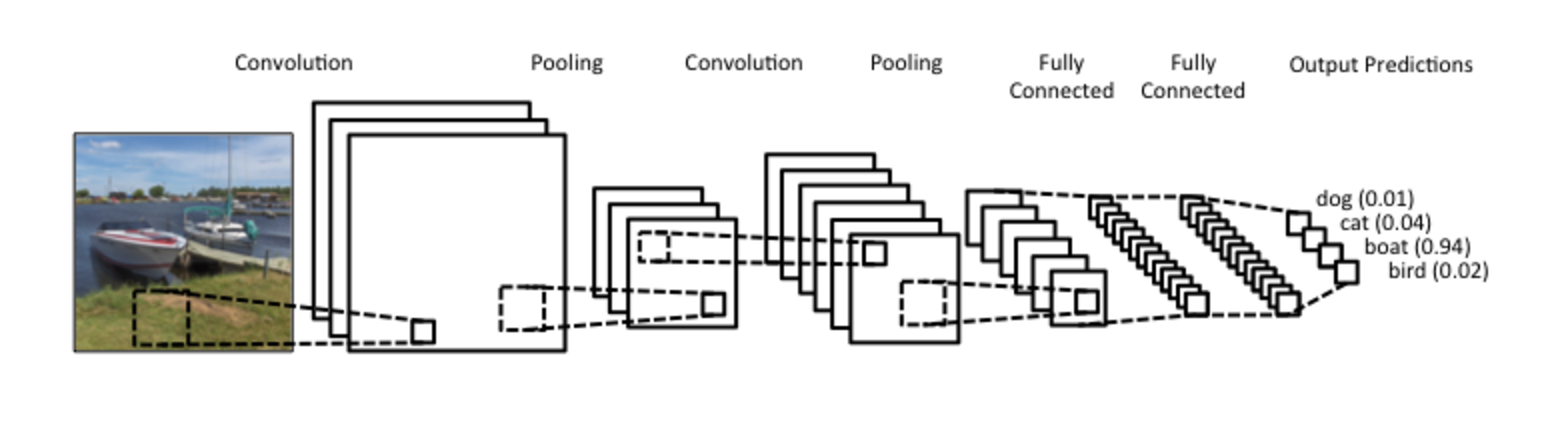
\includegraphics[scale=0.5]{fullstructure}
\end{center}
\subsection{Definition}
So now we have our full convolutional neural network. We take a raw image, and using filters, extract out features. We then use pooling to compress the data and repeat, generating features of features, and so on. We then feed all of these features into a fully connected standard neural network to classify an image based on this extracted, higher level information.

\end{document}
